\def\year{2019}\relax
\documentclass[letterpaper]{article} % DO NOT CHANGE THIS
\usepackage{aaai19}  % DO NOT CHANGE THIS
\usepackage{times}  % DO NOT CHANGE THIS
\usepackage{helvet} % DO NOT CHANGE THIS
\usepackage{courier}  % DO NOT CHANGE THIS
\usepackage[hyphens]{url}  % DO NOT CHANGE THIS
\usepackage{graphicx} % DO NOT CHANGE THIS
\urlstyle{rm} % DO NOT CHANGE THIS
\def\UrlFont{\rm}  % DO NOT CHANGE THIS
\usepackage{graphicx}  % DO NOT CHANGE THIS
\frenchspacing  % DO NOT CHANGE THIS
\setlength{\pdfpagewidth}{8.5in}  % DO NOT CHANGE THIS
\setlength{\pdfpageheight}{11in}  % DO NOT CHANGE THIS
\nocopyright
\graphicspath{{images/}}
%PDF Info Is REQUIRED.
% For /Author, add all authors within the parentheses, separated by commas. No accents or commands.
% For /Title, add Title in Mixed Case. No accents or commands. Retain the parentheses.
\pdfinfo{
/Title (Image Enhancement Applied to Dynamic Frame Generation)
/Author (Mark Wesley Harris)
} %Leave this	
% /Title ()
% Put your actual complete title (no codes, scripts, shortcuts, or LaTeX commands) within the parentheses in mixed case
% Leave the space between \Title and the beginning parenthesis alone
% /Author ()
% Put your actual complete list of authors (no codes, scripts, shortcuts, or LaTeX commands) within the parentheses in mixed case. 
% Each author should be only by a comma. If the name contains accents, remove them. If there are any LaTeX commands, 
% remove them. 

% DISALLOWED PACKAGES
% \usepackage{authblk} -- This package is specifically forbidden
% \usepackage{balance} -- This package is specifically forbidden
% \usepackage{caption} -- This package is specifically forbidden
% \usepackage{color (if used in text)
% \usepackage{CJK} -- This package is specifically forbidden
% \usepackage{float} -- This package is specifically forbidden
% \usepackage{flushend} -- This package is specifically forbidden
% \usepackage{fontenc} -- This package is specifically forbidden
% \usepackage{fullpage} -- This package is specifically forbidden
% \usepackage{geometry} -- This package is specifically forbidden
% \usepackage{grffile} -- This package is specifically forbidden
% \usepackage{hyperref} -- This package is specifically forbidden
% \usepackage{navigator} -- This package is specifically forbidden
% (or any other package that embeds links such as navigator or hyperref)
% \indentfirst} -- This package is specifically forbidden
% \layout} -- This package is specifically forbidden
% \multicol} -- This package is specifically forbidden
% \nameref} -- This package is specifically forbidden
% \natbib} -- This package is specifically forbidden -- use the following workaround:
% \usepackage{savetrees} -- This package is specifically forbidden
% \usepackage{setspace} -- This package is specifically forbidden
% \usepackage{stfloats} -- This package is specifically forbidden
% \usepackage{tabu} -- This package is specifically forbidden
% \usepackage{titlesec} -- This package is specifically forbidden
% \usepackage{tocbibind} -- This package is specifically forbidden
% \usepackage{ulem} -- This package is specifically forbidden
% \usepackage{wrapfig} -- This package is specifically forbidden
% DISALLOWED COMMANDS
% \nocopyright -- Your paper will not be published if you use this command
% \addtolength -- This command may not be used
% \balance -- This command may not be used
% \baselinestretch -- Your paper will not be published if you use this command
% \clearpage -- No page breaks of any kind may be used for the final version of your paper
% \columnsep -- This command may not be used
% \newpage -- No page breaks of any kind may be used for the final version of your paper
% \pagebreak -- No page breaks of any kind may be used for the final version of your paperr
% \pagestyle -- This command may not be used
% \tiny -- This is not an acceptable font size.
% \vspace{- -- No negative value may be used in proximity of a caption, figure, table, section, subsection, subsubsection, or reference
% \vskip{- -- No negative value may be used to alter spacing above or below a caption, figure, table, section, subsection, subsubsection, or reference

\setcounter{secnumdepth}{0} %May be changed to 1 or 2 if section numbers are desired.

% The file aaai19.sty is the style file for AAAI Press 
% proceedings, working notes, and technical reports.
%
\setlength\titlebox{2.5in} % If your paper contains an overfull \vbox too high warning at the beginning of the document, use this
% command to correct it. You may not alter the value below 2.5 in
\title{Image Enhancement Applied to Dynamic Frame Generation}
% Your title must be in mixed case, not sentence case. 
% That means all verbs (including short verbs like be, is, using,and go), 
% nouns, adverbs, adjectives should be capitalized, including both words in hyphenated terms, while
% articles, conjunctions, and prepositions are lower case unless they
% directly follow a colon or long dash
\author{Mark Wesley Harris\\ % All authors must be in the same font size and format. Use \Large and \textbf to achieve this result when breaking a line
% If you have multiple authors and multiple affiliations
% use superscripts in text and roman font to identify them. For example, Sunil Issar,\textsuperscript{\rm 2} J. Scott Penberthy\textsuperscript{\rm 3} George Ferguson,\textsuperscript{\rm 4} Hans Guesgen\textsuperscript{\rm 5}. Note that the comma should be placed BEFORE the superscript for optimum readability
University of Colorado Colorado Springs\\
wharris2@uccs.edu % email address must be in roman text type, not monospace or sans serif
}
\begin{document}

\maketitle

\begin{abstract}
One of the most applicable areas of machine learning to Computer Graphics is in the
generation of images. Image processing is very useful for graphics artists and
researchers, and may involve labeled or unlabeled data. We propose
a study of how machine learning can be applied to enahance the quality of an image.
4 different architectures are proposed to be studied, in the hopes of comparing
their results and finding the best possible architecture for enchancing images.
This research will be applied to a larger machine learning architecture that will be used to
speed up rendering of 3D animated feature films.
\end{abstract}

\section{Introduction}
\label{sec:introduction}
Rendering full-length feature films is a burdensome process
even for state-of-the-art equipment.
This is because the creation of each rendered frame is dependent upon the
complexity of the 3D environment and
efficiency of the chosen render engine.
%However, one may observe that for a majority of the time in any given animated sequence,
%neighboring frames contain gradual changes with smooth or predictable movements.
%Thus we should be able to predict what a frame will look like
%given enough data from the rest of the animated sequence.
Researchers are now turning to machine learning in order to improve
rendering and image processing performance.
However, there are many factors which make image generation difficult, including
the complexity of the image, the image context, and how the image will be used.
Recent research shows that we are able to obtain higher quality images by giving
an algorithm non-random seed data, such as a low-quality image, to generate from.
Proposed in this document is a study
on how to enhance low quality images using machine learning
as an application to image processing research in the field of Computer Graphics.

%Related work including fundamentals on image generation and enhancement is discussed.
%Then project related details are covered, following an explanation on how the project work
%will be evaluated and finally a timeline of work for this semester.

\section{Related Work}
\label{sec:related_work}
%\subsection{Image Processing}
%\subsubsection{Next Frame Prediction}
%Mahjourian \textit{et al.} \cite{next_frame_prediction}
%focus on generating the
%next frame of a monocular (i.e. single-view) video 
%given the video's previous frames. They deployed
%an LSTM machine learning model in order to generate a depth map representing the next frame.
%Another machine learning model was then applied to convert the generated depth
%map into the pixels of the predicted frame. The largest deficiency of the
%project was the poorness of the output frame's quality, as shown in Figure
%\ref{fig:frame_prediction}; in order to use their
%application for production-quality outputs, more steps would have
%to be taken to ensure the quality is comparable to the original input frames.
%
%\begin{figure}[htbp]
%\centerline{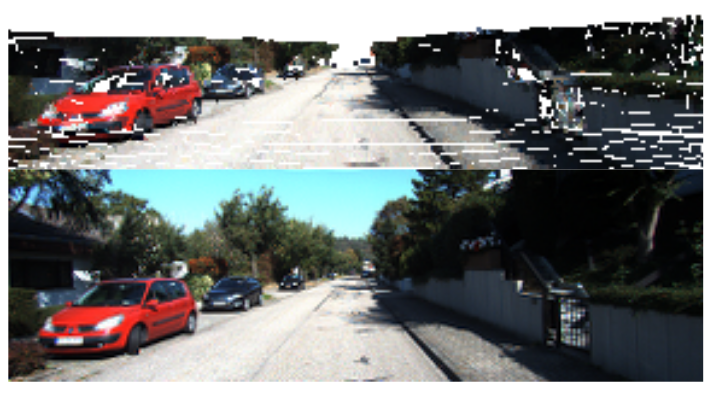
\includegraphics[width=8cm]{frame_prediction.png}}
%\caption{Example input (bottom) and output (top) of frame prediction algorithm
%\cite{next_frame_prediction}.}
%\label{fig:frame_prediction}
%\end{figure}
%
%The use of the LSTM model in order to
%collect changes from all previous frames instead of just one previous frame
%was most the noteworthy aspect of \cite{next_frame_prediction}.
%
%\subsubsection{Capsule Networks}
%2D Capsule Networks have been used to segment shape data in a
%more efficient way than the Convolutional Nueral Network (CNN) has
%done in the past. CNN's and other architectures
%``\dots often discard
%spatial arrangements in data, hence falling short of respecting
%the parts-to-whole relationship, which is critical to explain
%and describe 3D shapes'' \cite{3D_capsule_networks}.
%
%Sabour et al. \cite{dynamic_routing_capsules} introduced capsule networks (CapsNets) as a powerful
%alternative to CNNs, which learn ``\dots a more equivariant representation of images
%that is more robust to changes in pose and spatial relationships of parts of objects
%in images'' \cite{transforming_auto_encoders}.

\subsubsection{PG\textsuperscript{2}}
\label{subsubsec:pg2}
Ma \textit{et al.} 
present a system entitled
``Pose Guided Person Generation Network'', or PG\textsuperscript{2}
\cite{pose_guided_image_generation}.
This system takes as input a condition image, and a target image representing the pose
to be translated into (the choice of the representation for pose data is explained further in the
paper). Using a system of two generative models,
the algorithm produces as intermediate output a low-resolution
image that defines global structure and features, as well as a final refined
image of the person in the new pose. See Figure \ref{fig:pose_guided} for
a block diagram of their architecture.

\begin{figure}[htbp]
\centerline{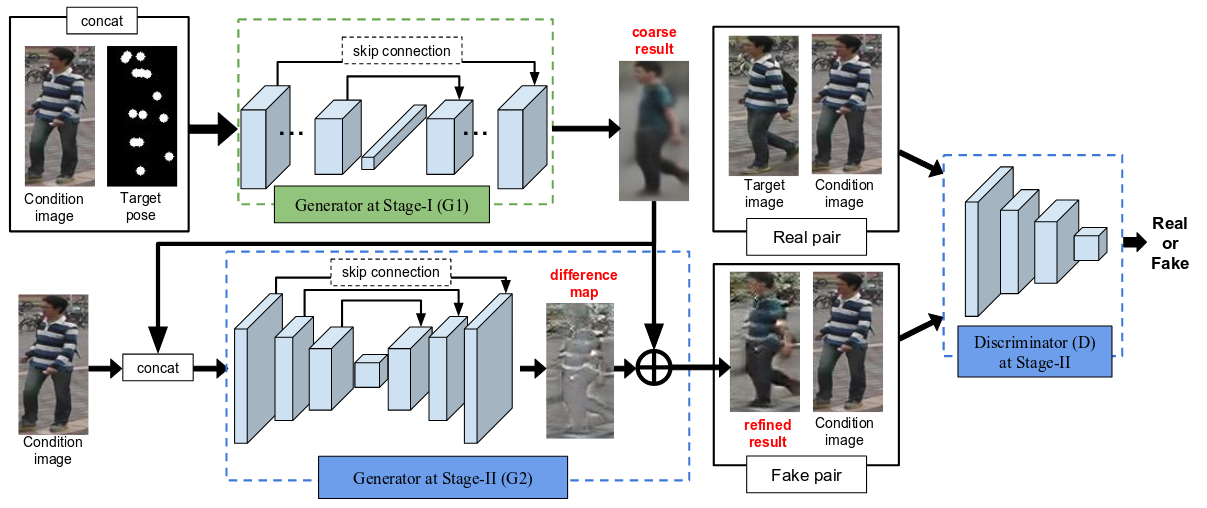
\includegraphics[width=8cm]{pose_guided.png}}
\caption{PG\textsuperscript{2} system architecture \cite{pose_guided_image_generation}.}
\label{fig:pose_guided}
\end{figure}

the final stage of PG\textsuperscript{2} \cite{pose_guided_image_generation}
takes as input a low quality structural image and
outputs a high resolution image of comparable quality to the target
(see G2 of Figure \ref{fig:pose_guided}).
They used a modified DCGAN \cite{unsupervised_learning}, which included
a generator and discriminator for training the model to export
high resolution versions of low quality images.
Example output of their architecture given the condition image and a new pose
is shown in Figure \ref{fig:pg2_results}.

\begin{figure}[htbp]
\centerline{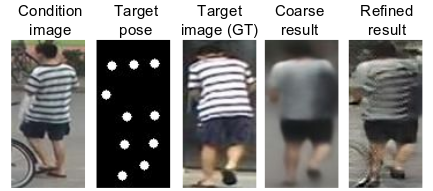
\includegraphics[width=8cm]{pg2_results.png}}
\caption{PG\textsuperscript{2} Example Output \cite{pose_guided_image_generation}.}
\label{fig:pg2_results}
\end{figure}

%\subsection{Image Enhancement}
%\label{subsec:image_enhancement}
%\subsubsection{Low to High Sampling}
%Schied \textit{et al.}
%generated high quality outputs given very low quality input
%images \cite{spatiotemporal}. The inputs of their algorithm are renderings using one path-per-pixel global
%illumination. As shown in Figure \ref{fig:spatiotemporal}, they are able to
%transform very crude, noisy frames into production-grade outputs comparable to
%the frames rendered at full resolution. Their algorithm is essentially a
%multi-pass filter which the inputs are fed into, making it very fast and
%reliable.
%
%My thesis work requires frame generation given scene data that has not yet been rendered,
%while \cite{spatiotemporal} depends on the input of entire rendered frames.
%However, there may be other components of their research that can be extracted
%to benefit the work proposed here.
%
%\begin{figure}[htbp]
%\centerline{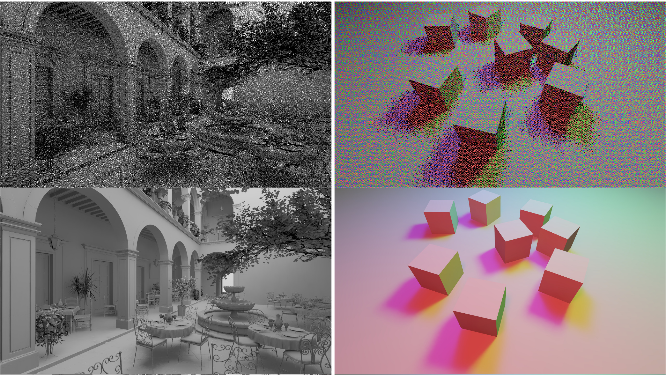
\includegraphics[width=8cm]{spatiotemporal.png}}
%\caption{Spatiotemporal Variance-Guided Filtering \cite{spatiotemporal}.}
%\label{fig:spatiotemporal}
%\end{figure}
%
%\subsubsection{PG\textsuperscript{2}}
%As mentioned in the preceeding section,
%the final stage of PG\textsuperscript{2} \cite{pose_guided_image_generation}
%takes as input a low quality structural image and
%outputs a high resolution image of comparable quality to the target
%(see G2 of Figure \ref{fig:pose_guided}).
%They used a modified DCGAN \cite{unsupervised_learning}, which included
%a generator and discriminator for training the model to export
%high resolution versions of low quality images.
%Example output of their architecture given the condition image and a new pose
%is shown in Figure \ref{fig:pg2_results}.
%
%\begin{figure}[htbp]
%\centerline{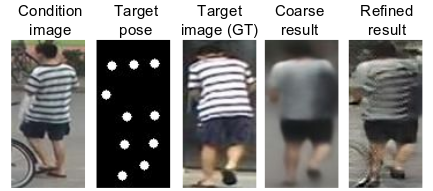
\includegraphics[width=8cm]{pg2_results.png}}
%\caption{PG\textsuperscript{2} Example Output \cite{pose_guided_image_generation}.}
%\label{fig:pg2_results}
%\end{figure}

\subsection{Applicable Architectures}
\subsubsection{DCGAN}
Goodfellow \textit{et al.} first proposed the Generative Adversarial Network (GAN)
as a way to train a model to produce more realistic images
\cite{generative_adversarial_networks}.
The network is made up of two architectures:
a generator, G, and a disciminator, D.
GAN's are able to generate new images that have similar qualities to
those in the dataset which they are trained on.
Radford \textit{et al.} first proposed the Deep Convolutional Generative Adversarial Network (DCGAN),
which is similar to the GAN
but uses convolutional and convolutional-transpose layers in D and G, respectively
\cite{unsupervised_learning}.

Ma \textit{et al.} were successful in using
a variant conditional DCGAN as their G2 model, which is similar to the work proposed here
\cite{pose_guided_image_generation}.
See Figure \ref{fig:pg2_results} for example outputs of their algorithm.
A Pytorch implementation for the DCGAN is stored on GitHub
\cite{dcgan_git}. This repository is explained thoroughly in a walkthrough
in Pytorch documentation \cite{dcgan_example}.

\subsubsection{PixelCNN++}
PixelCNN is a Convolutional Neural Network that is conditioned on an input image
\cite{conditional_image_generation}.
The architecture uses the input image vector to generate output images similar to it.
PixelCNN++ \cite{pixelcnn++} is a project developed by researching the
PixelCNN architecture with improvements made
for system efficiency and image output.
Implementation for the PixelCNN++ architecture can be found on GitHub \cite{pixelcnn++_git}.
Example outputs of their implementation are shown in Figure \ref{fig:pixelcnn++}.

\begin{figure}[htbp]
\centerline{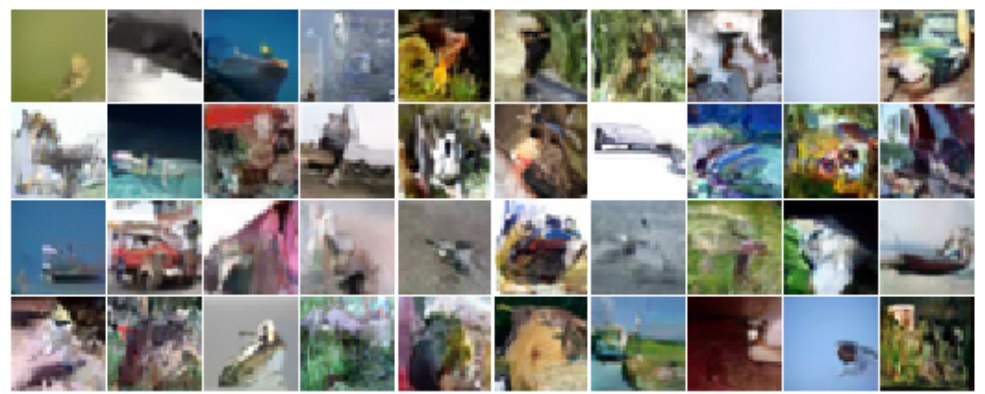
\includegraphics[width=8cm]{pixelcnn++.png}}
\caption{PixelCNN++ Example Outputs \cite{pixelcnn++}.}
\label{fig:pixelcnn++}
\end{figure}

\subsubsection{Pix2Pix}
Pix2Pix was a system designed by Isola \textit{et al.} 
as a tool to help artists and designers take advantage of processing images with machine learning
\cite{image_to_image}.
They found their model worked well in synthesizing, reconstructing, and colorizing
input images, as shown in Figure \ref{fig:image_to_image}.
The architecture is a conditional GAN (cGAN) which is similar to the DCGAN above, however
the input vector is random noise instead of a condition image.
Implemenation for the Pix2Pix architecture can be found on GitHub
\cite{pix2pix_git}.

\begin{figure}[htbp]
\centerline{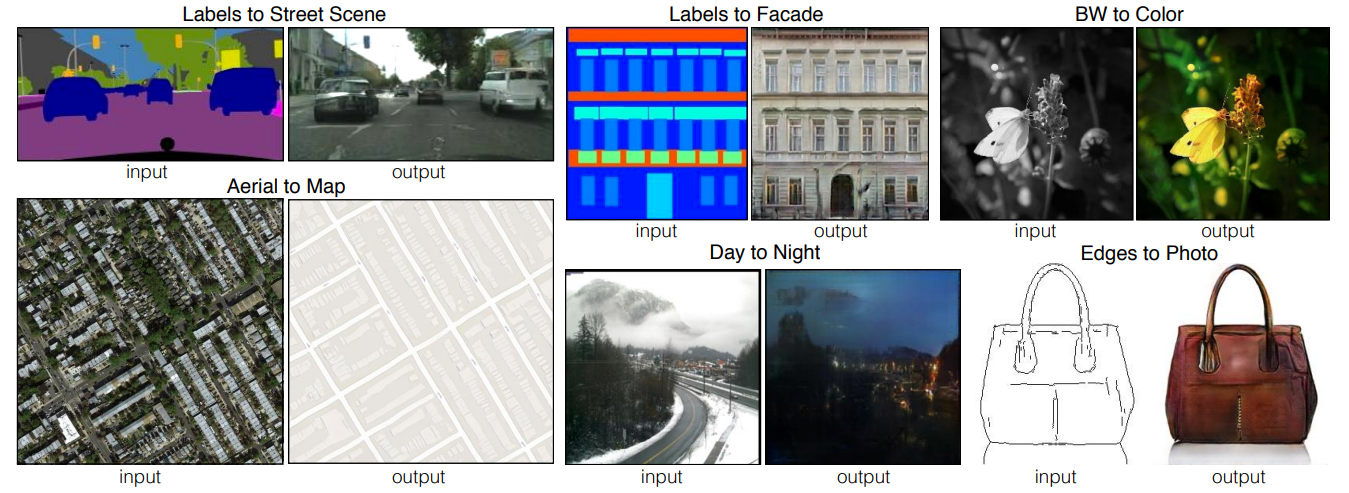
\includegraphics[width=8cm]{image_to_image.png}}
\caption{Image-to-Image Translation Example Outputs \cite{image_to_image}.}
\label{fig:image_to_image}
\end{figure}

\subsubsection{Sparse Attention}
Sequence to sequence \cite{generative_transformers}.
The Sparse Attention results (shown in Figure \ref{fig:sparse_attention}) are
much higher quality than the PixelCNN++ results and possibly
the DCGAN results.
Implementation for the Sparse Attention system can be found on GitHub
\cite{sparse_attention_git}.

\begin{figure}[htbp]
\centerline{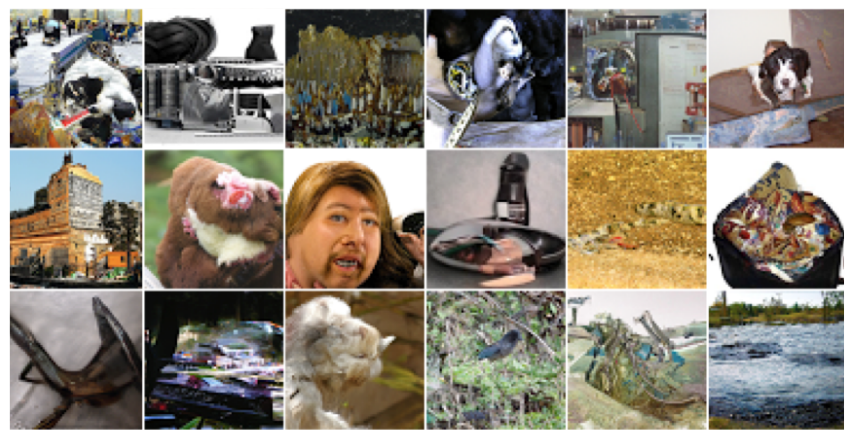
\includegraphics[width=8cm]{sparse_attention.png}}
\caption{Sparse Attention Example Outputs \cite{generative_transformers}.}
\label{fig:sparse_attention}
\end{figure}

\section{Proposed Work}
\label{sec:proposed_work}
\subsection{Dataset Creation}
\label{subsec:data}
We have developed an algorithm to deconstruct frames from an animated sequence
and compile them into a database of image blocks to be processed for the
training dataset.
A frame is first broken into
small (32 x 32 pixel) sections, referred to as ``frameblocks''.
Frameblocks representing a majority of change between two frames
are selected as part of the base dataset.
This process ensures that all images generated for the dataset
are representative of what is animated and that they are generally unique
in comparison to each other.
Figure \ref{fig:frameblock_generation} compares how material attributes
(such as transparency and reflection) may alter which frameblocks are selected.
The frameblocks outlined in red are
included in the dataset while frameblocks outlined in blue are not.

\begin{figure}[htbp]
\centerline{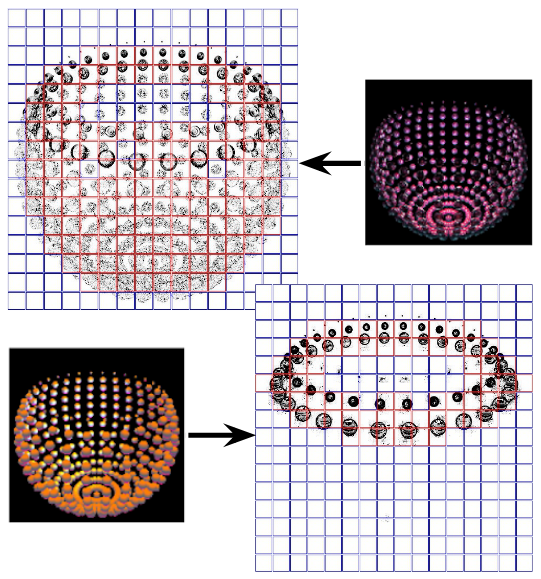
\includegraphics[width=8cm]{frameblock_generation.png}}
\caption{Frameblock generation between scenes with different attributes.}
\label{fig:frameblock_generation}
\end{figure}

A 13 second long animation (300 frames each with 1920 x 1080 pixels) was fed into the program,
resulting in a collection of 14,330 frameblocks (32 x 32 pixels).
In order to create the training dataset, these images will be
made into similar quality
to the intermediate output of Generator I 
in the PG\textsuperscript{2} architecture
(Figure \ref{fig:pose_guided}) \cite{pose_guided_image_generation}.
The training dataset will be blurred and small anomolies will be added uniformly
such that a general structure can be seen but no details are visible.
Copies of the original frameblocks are kept to form an image pair that can be used
as validation for the discriminator.
See Figure \ref{fig:training_pair} for examples of structural images
compared to their full-resolution counterparts.

\subsubsection{Dataset Validation}
Since this dataset has not been previously tested, one may conjecture that there are
concerns of over-fitting; as discussed by Radford \textit{et al.},
``as visual quality of samples from generative image models has improved, concerns of
over-fitting and memorization of training samples have risen''
\cite{unsupervised_learning}.
However, the dataset creation algorithm was created with overfitting in mind.
The algorithm only exports frameblocks which exceed a certain threshold in change
between frames or frame sets. Thus, it is unlikely similar frameblocks will be exported,
and generally each frame block is unique to its position relative to other objects in the scene.

If over-fitting does occur,
the dataset algorithm can be altered.
We also plan to test with other datasets in order to verify the results with applicable benchmarks
and improve the evaluation of the developed architecture.

\subsection{Model Construction}
\label{subsec:model}
The architectures applicable to this project are enumerated below.
As time allows, each architecture will be implemented, evaluated, and compared
against. The conclusion of this project will be an explanation of which architectures performed the best
for the given problem.
\begin{enumerate}
\item \textbf{DCGAN} --
Rate, dataset, \cite{dcgan_git}.
\item \textbf{Pix2Pix} --
Rate, dataset, \cite{pix2pix_git}.
\item \textbf{Sparse Attention} --
Rate, dataset, \cite{sparse_attention_git}.
\item \textbf{PixelCNN++} --
The PixelCNN++ architecture will be looked at last, since it has the expected lowest
quality outputs after training.
Rate, dataset, \cite{pixelcnn++_git}.
\end{enumerate}

\section{Evaluation}
\label{sec:methods/evaluation}
The implemented architectures will be evaluated on how well they are able to learn how to
enhance an altered image. After optimization and training have taken place,
an altered image within the unknown test dataset will be input into the algorithm, and the output
will be compared to the original image. An example input data and the expected output
of the algorithm is shown in Figure \ref{fig:training_pair}.

\begin{figure}[htbp]
\centerline{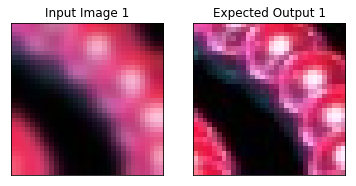
\includegraphics[width=7cm]{training_pair_1.png}}
\centerline{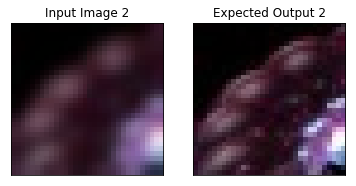
\includegraphics[width=7cm]{training_pair_2.png}}
\caption{Example of inputs (left) and expected outputs (right) of the proposed work.}
\label{fig:training_pair}
\end{figure}

A difference map (XOR) will be taken between the image output of the algorithm
and original image, in order to calculate a percentage difference between them.
Various frameblocks will be tested to determine how well the architecture fairs for the frame
as a whole.

\section{Semester Timeline}
\label{subsec:semester_plan}
\textbf{\textit{9/16 -- 9/23} Environment Setup (1 week)}
\begin{itemize}
\item Get PyTorch working.
\item Test on sample code architectures (DCGAN, cGAN, CNN, and Transformer).
\end{itemize}
\textbf{\textit{9/23 -- 10/7} DCGAN Architecture (2 weeks)}
\begin{itemize}
\item Run the sample code.
\item Make edits.
\end{itemize}
\textbf{\textit{10/7 -- 10/21} Documentation for Midterm Presentation (2 weeks)}
\begin{itemize}
\item 7 - 10 references, 4 - 5 pages, 7 - 10 minutes.
\end{itemize}
\textbf{\textit{10/21 -- 10/28} Midterms Wiggle Room (1 week)}
\textbf{\textit{10/28 -- 11/11} Transformer Architecture (2 weeks)}
\begin{itemize}
\item Run the sample code.
\item Make edits.
\end{itemize}
\textbf{\textit{11/11 -- 11/25} cGAN Architecture (2 weeks)}
\begin{itemize}
\item Run the sample code.
\item Make edits.
\end{itemize}
\textbf{\textit{11/25 -- 12/2} Thanksgiving Break (1 week)}
\begin{itemize}
\item Make comparisons based on previous work and start drawing conclusions.
\end{itemize}
\textbf{\textit{12/2 -- 12/9} Documentation for Final Presentation (1 week)}
\begin{itemize}
\item 6 - 8 pages, 10 - 15 minutes.
\end{itemize}
\textbf{\textit{12/9 -- 12/16} Finals Wiggle Room (last week)}

\section{Conclusion}
\label{sec:conclusion}
In this document is proposed work on an image enhancement algorithm as
part of an overall machine learning architecture for dynamically
generating rendered frames. The architecture is modeled off of work from
Ma \textit{et al.} and their PG\textsuperscript{2} system
\cite{pose_guided_image_generation}.
The proposed model construction and evaluation is taken from
the DCGAN \cite{unsupervised_learning},
CNN \cite{pixelcnn++},
cGAN \cite{image_to_image},
and Transformer \cite{generative_transformers} architectures.
The best solution for the presented problem will be found
by comparing the outputs of these models.

\nocite{pixel_recurrent}
\nocite{parallel_density}
\nocite{pixel_snail}
\nocite{pixel_subscale}
%\nocite{next_frame_prediction}
%\nocite{combining_multiple_cnn}
%\nocite{deep_video_prediction}
%\nocite{fusionnet}
%\nocite{show_and_tell}
%\nocite{pose_cnn}

\bibliography{proposal}
\bibliographystyle{aaai}

\end{document}
